\title[JASA/draft]{Under-ice acoustic navigation using real-time model-aided range estimation}
\author{EeShan C. Bhatt}
\email{ebhatt@whoi.edu}
\affiliation{MIT-WHOI Joint Program in Oceanography/Applied Ocean Science \& Engineering, Cambridge and Woods Hole, MA, USA}
\affiliation{Department of Mechanical Engineering, Massachusetts Institute of Technology, Cambridge, MA}
\author{Oscar Viquez}
\affiliation{Department of Mechanical Engineering, Massachusetts Institute of Technology, Cambridge, MA}
\author{Henrik Schmidt}
\email{henrik@mit.edu}
\affiliation{Department of Mechanical Engineering, Massachusetts Institute of Technology, Cambridge, MA}


% \author{Author Four}
% \email{author.four@university.edu}
% \affiliation{Department2,  University2, City, State ZipCode, Country}

\preprint{Bhatt, JASA}   %  if you want want this message to appear in upper right corner of title page

\date{\today}

\begin{abstract}
Almost all underwater navigation paradigms rely on the conversion of recorded travel time into range to compute a trilateration solution.
For real-time navigation, this conversion is treated deterministically.
For positioning in post-processing, more computationally and/or labor intensive modeling methods are often employed to reduce the uncertainty driven by multipath arrivals.
An autonomous underwater vehicle deployment in March 2020 in the Beaufort Sea faced significant operational challenges with a total ice-covered environment and complex acoustic propagation via the Beaufort Lens.
We implement an embedded, stochastic, ray-based prediction of the horizontal group velocity and validate its performance with communication events between GPS-aided beacons, achieving a pseudorange mean absolute error of 11 m.
In post-processing, we introduce a multipath criterion and achieve ranging performance that rivals GPS.
To our knowledge, these results are the first field experiment to demonstrate a real-time, physics-based data processing to minimize ranging error in underwater navigation.
\end{abstract}

%% pacs numbers not used

\maketitle

\newcommand{\llabel}[1]{\hypertarget{llineno:#1}{\linelabel{#1}}}
\newcommand{\lref}[1]{\hyperlink{llineno:#1}{\ref*{#1}}}

% =========================================================================== %
% =========================================================================== %

\section{Introduction}
\label{sec:1}  

Autonomous underwater vehicles (AUVs) are an increasingly capable platform to explore and sample the ocean, particularly for remote and/or dangerous environments.
Lightweight, mobile, and inexpensive compared to crewed and ship-based systems, these vehicles can enable a safer, data-forward style of field oceanography \citep{bellingham_robotics_2007,petillot_underwater_2019}.

\llabel{test}

But navigation uncertainty is a major challenge in considering AUVs as reliable and standard tools for oceanographic research.
While land and air-based robots utilize satellite-based global positioning system (GPS) to achieve stunning location accuracy and precision throughout the duration of their missions, AUVs cannot access GPS while underwater due to the rapid attenuation of electromagnetic waves \citep{preisig_acoustic_2007}.
A vehicle can stall on the surface to receive a GPS fix, but this foolproof method of re-positioning is inaccessible in an ice-covered environment or other GPS-denied situations.
A recent study tracking 22 floats under the ice in the Weddell Gyre near Antarctica showed that they were unable to surface for 8 months and position uncertainty grew to 116 $\pm$ 148 km in the lateral directions \citep{chamberlain_observing_2018}.

\llabel{test2}

Much progress has been made in underwater vehicle navigation, which relies on any combination of dead reckoning, hydrodynamic models, inertial navigation systems, doppler velocity logs, and/or acoustic baseline navigation systems \citep{paull_auv_2014}.
In particular, the long baseline (LBL) navigation system is the most similar in scale and style to GPS, and most appropriate for mitigating drift in underwater vehicle localization without overburdening computation on the vehicle \citep{van_uffelen_global_2021}.

\subsection{Timing, Positioning, and Navigation}

Underwater acoustic navigation (and GPS) is predicated on timing and positioning.
Timing is the ability to maintain accurate and precise time, sometimes synchronized across multiple nodes.
The advent of the WHOI micro-modem \citep{singh_underwater_2006} and synchronized chip scale atomic clocks \citep{gardner_second_2016} enabled ranging via one-way travel time (OWTT).

Positioning is the ability to accurately determine one's location and is generally done via trilateration.
Navigation assumes a degree of autonomy to move from a current position to a desired one.
The standard for real-time navigation efforts assume a locally homogeneous sound speed profile (SSP) that enables a linear, deterministic scaling between travel time and range \citep{eustice_recent_2006,eustice_experimental_2007,webster_preliminary_2009,webster_advances_2012}.
Short range (less than ten kilometers) navigation efforts achieve minimal navigation error with a nominal sound speed value \citep{eustice_experimental_2007,webster_preliminary_2009,kepper_mems_2017}.
For mesoscale (tens to hundreds of kilometers) navigation efforts, a deterministic \citep{graupe_preliminary_2019} or through-the-sensor \citep{webster_towards_2015} value for sound speed is used, but error remains in the hundreds of meters.

Post-processing localization efforts (re-navigation for a self-determinedly moving object or re-positioning for a passively moving one), without computational or time constraints, can indulge more complex acoustic methods and/or ocean representations.
There are many different approaches, from considering a temporally averaged mean depth dependent SSP \citep{van_uffelen_localization_2016}, including spatio-temporal variability in the sound speed profile to minimize error \citep{graupe_preliminary_2019, mikhalevsky_deep_2020}, comparing acoustic records with synthetic acoustic records computed through an ocean model \citep{wu_deep_2019}. 
The ``cold start'' algorithm developed by \citet{mikhalevsky_deep_2020} isolates a specific ray path to find a representative group velocity and re-positioned a floating hydrophone array with an error of 85 m and a standard deviation of 32 m relative to ground truth GPS data, but implementing this algorithm for navigation remains to be seen.
These post-processing efforts have generally been deemed too computationally intensive and/or labor intensive for real-time efforts, where automation of identifying time arrivals is further complicated by multipath. 

\subsection{Underwater positioning and navigation in the Arctic}

Underwater navigation research is broadly motivated by GPS-like navigation in GPS-denied conditions.
The Arctic, while remote, is the perfect place to test mature navigation technologies in real GPS-denied conditions.

Literature and historical reviews of underwater navigation approaches in under-ice conditions highlight the emerging technology learning curve for vehicle operations in the Arctic, the hostile conditions brought on by a semi-permanent moving ice cover, and the need for both absolute and relative navigation with little to no tolerance for error \citep{norgren_unmanned_2014,mcfarlane_autonomous_2015,barker_scientific_2020}.

One of the first successful AUV launches and recoveries involved equipping the vehicle with barbs which became entangled into a homing net underneath the ice \citep{bellingham_auv_1993}.
Since then, AUVs have been used for ocean bottom \citep{jakuba_long-baseline_2008,kunz_deep_2008}, under-ice \citep{kaminski_12_2010}, and hydrographic surveys \citep{kukulya_under-ice_2010,kukulya_development_2016,stevens_linking_2016,plueddemann_autonomous_2012}.
These efforts show a combination of short and long range positioning systems, where all acoustic navigation methods used a depth-averaged sound speed for linear scaling between recorded travel time and range.
In many cases robust quantitative navigation performance could not be evaluated due to small operational scale and/or moving ice floes.
But most importantly, all of these efforts experienced a nearly isovelocity or classical upward refracting Arctic acoustic environment.

The new Arctic\textemdash one with much less multi-year sea ice\textemdash is experiencing significant changes in the water column as well \citep{mackinnon_warm_2021}.
The Beaufort Lens is a highly dynamic, highly stratified water mass, keeping a neutrally buoyant layer of warm Pacific water at 50 to 70 m in depth.
Surrounded by cooler waters, it distinguishes a local maximum in the SSP, creating an upper and lower duct\textemdash the upper duct degrades signal coherence due to intensified ice interaction and the lower duct effectively traps sound for long range propagation \citep{poulsen_acoustic_2016}. 
Modeling output \citep{duda_long-range_2019,duda_effects_2021} and experimental observations \cite{kucukosmanoglu_observations_2021,badiey_azimuthal_2019,ballard_temporal_2020} indicate a high degree of spatio-temporal variability of the lower duct throughout the Chukchki and Beaufort Seas.

An experiment in 2014 exploited this lower duct to provide acoustic navigation and communication at mesoscale ranges in the Canada Basin.
\citet{freitag_long_2015} and \citet{webster_towards_2015} deployed multiple GPS-linked ice buoys with transducers that were capable of communications greater than 400 km with a range accuracy of 40 m when the sound speed was known.
The transducers were at 100 m depth, well-positioned in the lower duct spanning 50 to 200 m.
The glider navigation accuracy, however, was severely degraded as acoustic packets were sent when the gliders were outside the sound channel.
When gliders were deployed again in 2017, their navigation error was on the order of half a kilometer, and a glider re-navigation using an acoustic arrival method and the average sound-speed profile from the gliders reduced navigation error by a factor of 4-5, depending on the dive \citep{graupe_preliminary_2019}.
Navigation error is referenced to intermittent GPS fixes, as all of these glider deployments occurred in the Marginal Ice Zone with little to no ice at the time.

\subsection{Ice Exercise 2020}

The Beaufort Lens is equally important for shorter ranges as well, where a shadow zone over vehicle operational ranges is created by a drastic change in the reliable acoustic path \citep{schmidt_acoustic_2016}.
Thus the key simplifying assumption for OWTT ranging\textemdash a locally homogeneous sound speed profile that enables a linear, deterministic scaling between travel time and range\textemdash becomes more inaccurate due to increased multipath in the upper duct of the Beaufort Lens.

The results from this paper derive from data taken while deploying AUV Macrura, a modified Bluefin-21, during the Ice Exercise 2020 (ICEX20), in the Beaufort Sea, in March 2020.
The challenges anticipated for ICEX20\textemdash total ice cover, moving ice floes, and a variable Beaufort Lens\textemdash crystallized the necessity of environmental awareness for the navigation solution.

In this paper we present a working solution for underwater navigation that achieves GPS-like accuracy and precision.
We embed a stochastic prediction of a single group velocity to convert recorded travel time into range.
This prediction ingests an updatable snapshot of the SSP via acoustic message; over the course of ICEX20, this capability was used several times. 
Ultimately, integrating environmental realism enabled a successful emergency recovery of the AUV.
Due to a harddrive error, the AUV stalled underneath the ice surface and broadcasted its location.
A team was able to dig a hole through the 2 meter ice sheet and immediately see the vehicle.
Its successful recovery amidst total ice cover is shown in Fig. \ref{fig:vehicleRecovery}.
\begin{figure}[h!]
	\centering
	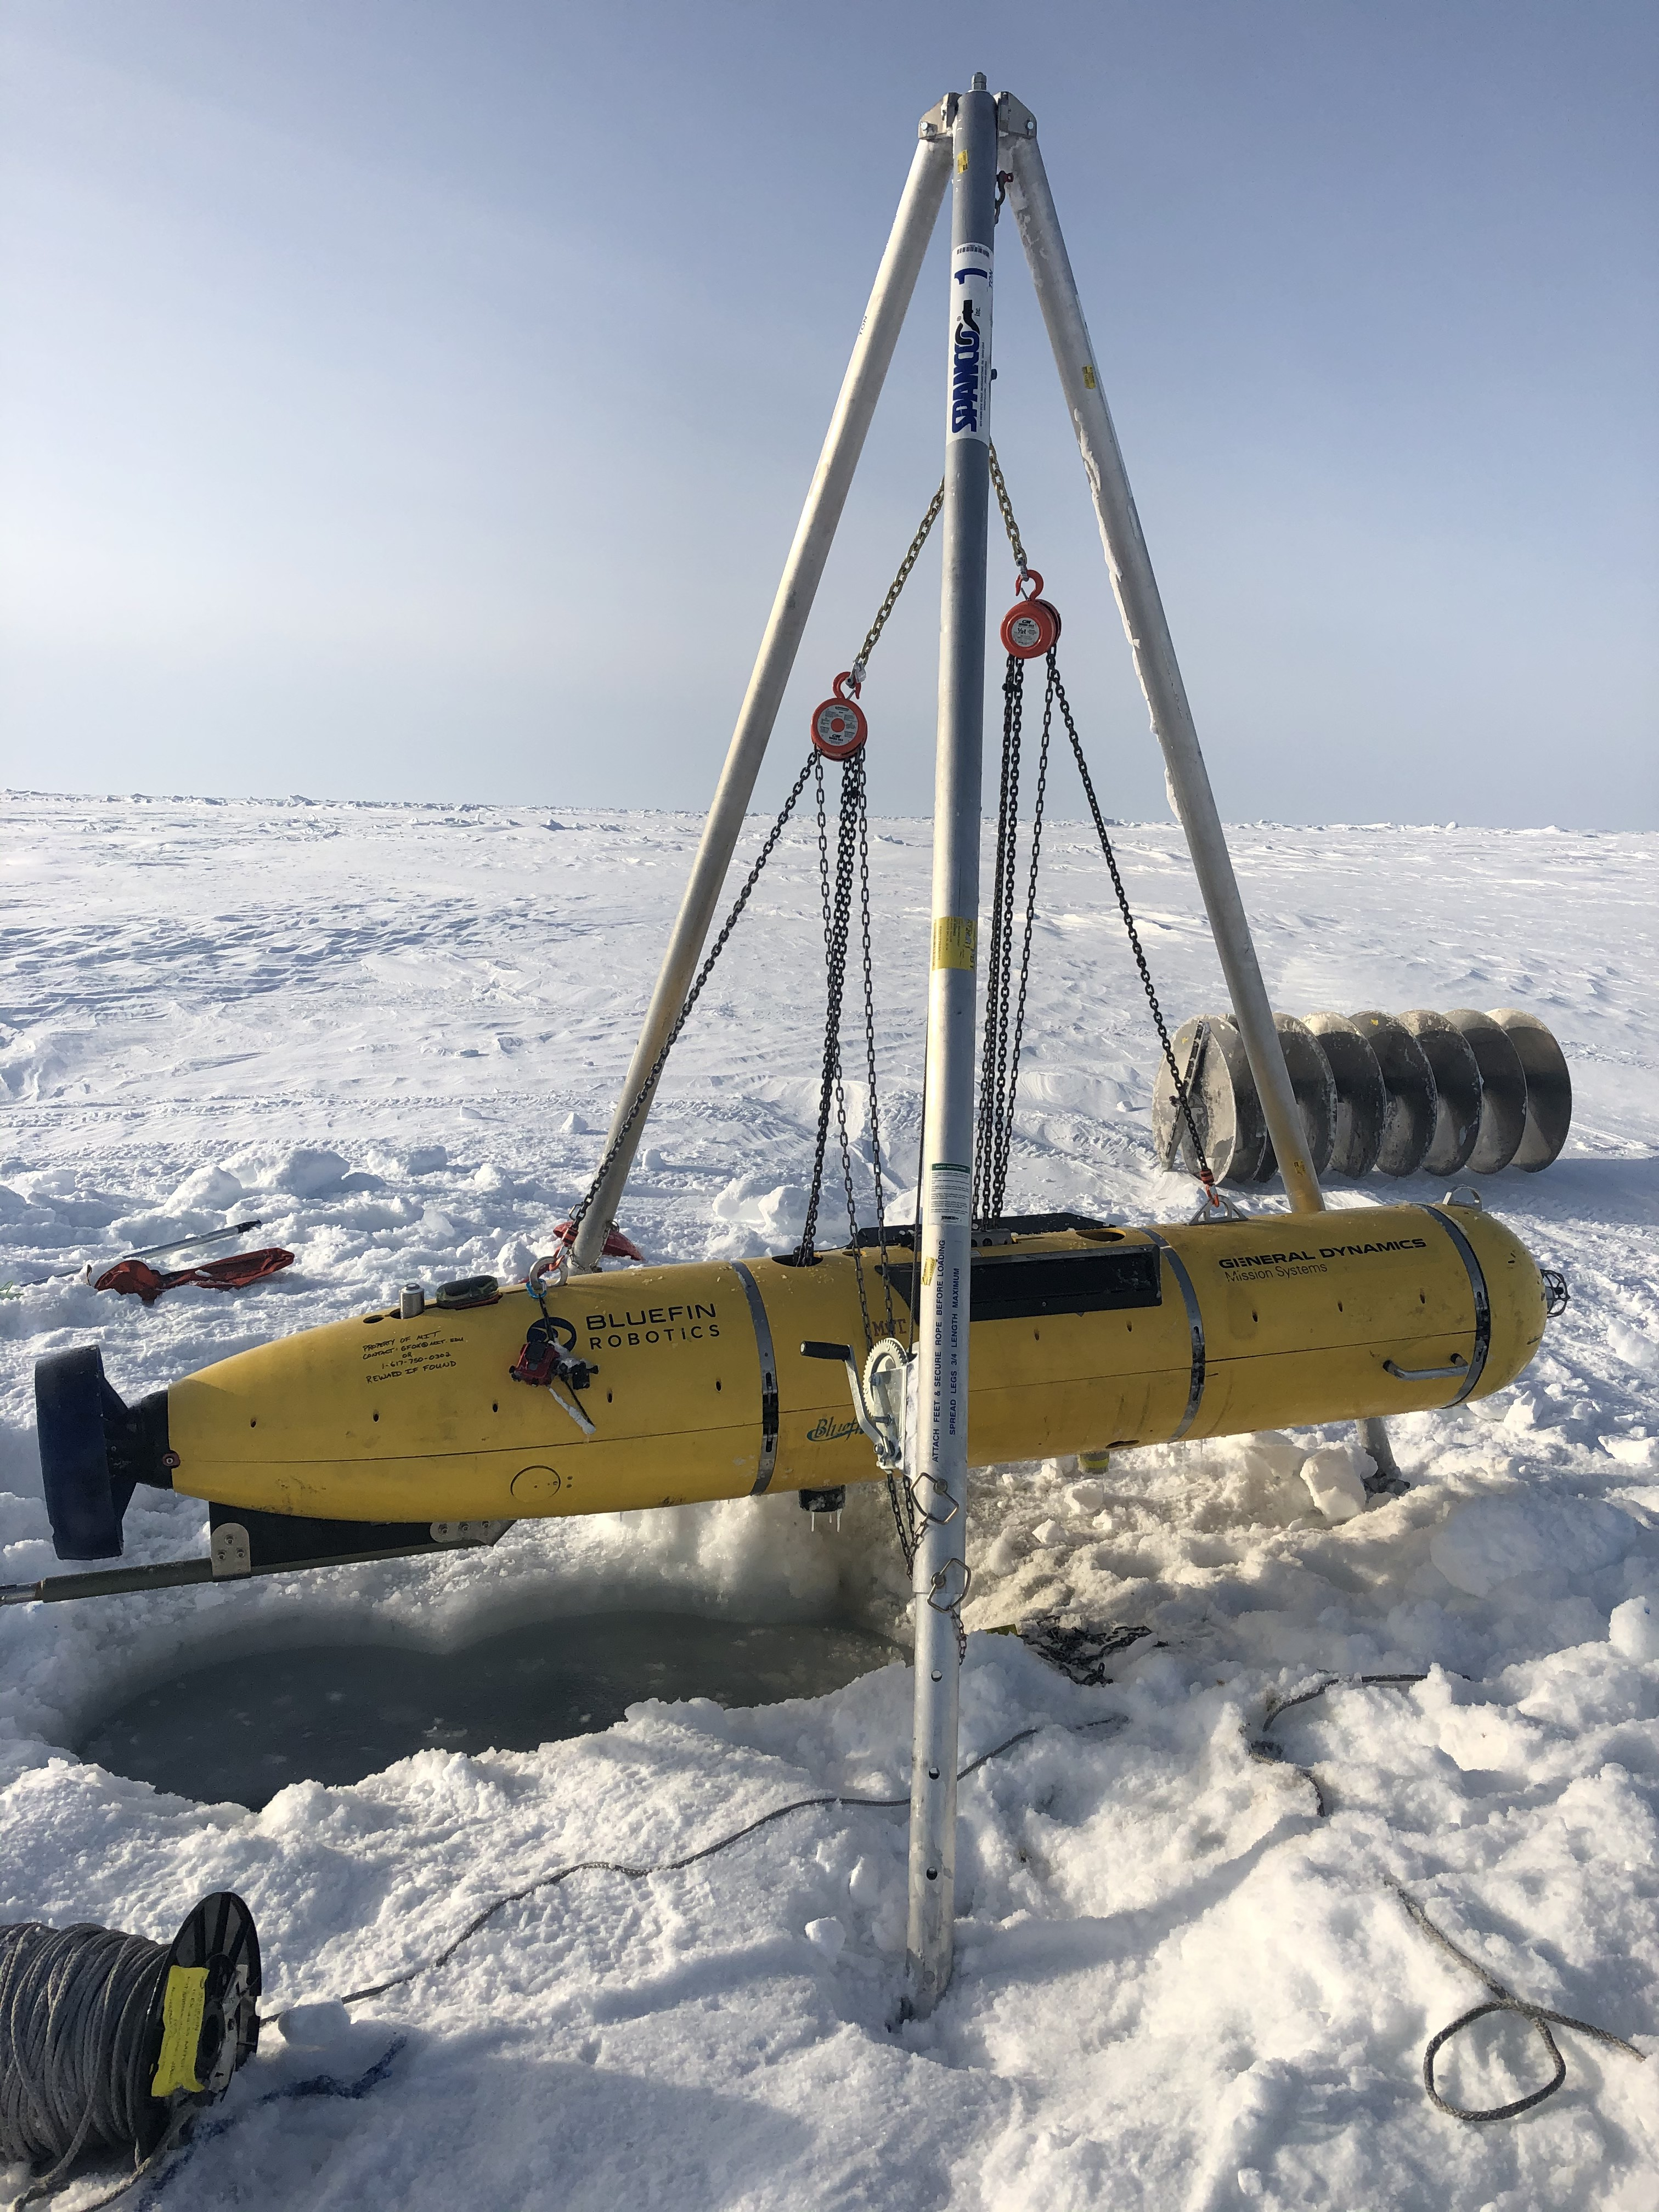
\includegraphics[width=\reprintcolumnwidth]{figs/Fig1.jpg}
	\caption{The successful emergency recovery of AUV Macrura, with the the auger used to drill through the ice sheet in the background. Photo courtesy of LT CDR D. Goodwin.}
	\label{fig:vehicleRecovery}
\end{figure} 

The rest of this paper is organized as follows: Section~\ref{sec:methods} presents the physical
experimental setup and model-based data processing; 
section \ref{sec:realtime} quickly conveys real-time results and the limitations of the data collected; section~\ref{sec:postprocess} presents key results for group velocity predictions and range estimations; section~\ref{sec:discussion} closes with a discussion on importance, future work, and broader relevance.

% =========================================================================== %
% =========================================================================== %
\section{Methods}
\label{sec:methods}

The acoustic communication dataset accrued for ICEX20 relied on the Integrated Communication and Navigation Network (ICNN) \citep{schneider_self-adapting_2020,randeni_construction_2020,randeni_high-resolution_2021}.
The ICNN was initially developed via numerous virtual experiments, to push the boundaries of algorithms and interfaces between different hardware components.
The simulation approach is a necessary testbed for robustness and produces better results than post-processing previous field data, as that restricts mission configurations to the data taken, which can hamper troubleshooting in the field.
The simulation capabilities are largely physics-driven with a modular system of systems approach: an environmental simulator with sub-components for the ocean, including Arctic ice drift and ocean acoustic propagation; a vehicle simulator with sub-components for vehicle dynamics and navigation; a topside hardware simulator and acoustic communications simulator, both with a software-only configuration and a hardware-in-the-loop version \citep{schneider_netsim_2018}.
The virtual environment similarly emulates the interfaces between the real components to test the entire software pipeline.
Both simulation capabilities are integral to mission success.

\subsection{Operational paradigm on the ice}

The ICNN is comprised of four ice buoys, in a loose rectangle, roughly 2 km away from a central ice camp with a topside computer, as shown in Fig.~\ref{fig:icnnOverview}.

\begin{figure}[h!]
	\centering
	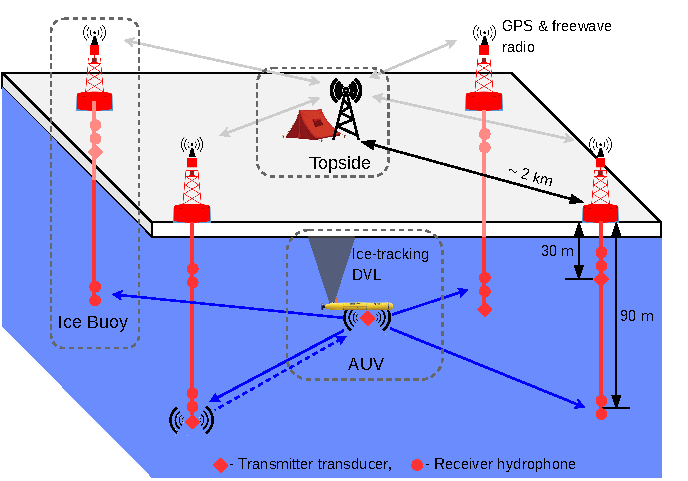
\includegraphics[width=\reprintcolumnwidth]{figs/Fig2.pdf}
	\caption{A schematic overview of the Integrated Communication and Navigation Network (ICNN), which provides joint data-transfer and tracking between AUV and a human decision maker at Topside.}
	\label{fig:icnnOverview}
\end{figure}

Each ice buoy is outfitted with a WHOI Micro-Modem \citep{singh_underwater_2006}, with a four-element receiver array and a single transmitter, and one-tenth of a millisecond resolution.
The receiving and transmitting elements were split between shallow and deeper depths (30 and 90 m, respectively) to provide better coverage due to the acoustic shadow zone in the Beaufort Lens.
The buoys do not encompass the full operating range of the vehicle but are positioned to minimize overlap in trilateration for spherical positioning \citep{deffenbaugh_relationship_1996}.

Vehicle missions in any underwater environment, but especially acoustically complex ones, must balance competing uses of the acoustic channel.
This network uses a single synchronized digital communication packet to provide both tracking and data to the operator.
The ICNN operational paradigm is as follows:
\begin{enumerate}
\item The AUV, running an ice-tracking DVL and an onboard hydrodynamic model, broadcasts its perceived location on a scheduled, time-synchronized message via WHOI Micro-Modem
\item Four ice buoys, each outfitted with a WHOI Micro-Modem, receive messages from the AUV and send that information over freewave radio to a Topside computer
\item The topside computer converts travel times into range estimates using a stochastic embedded prediction of the horizontal group velocity via BELLHOP ray tracing code \citep{porter_bellhop_2011} coupled with a Virtual Ocean \citep{schneider_netsim_2018}
\item The topside computer calculates a new position by trilaterating the range estimates
\item The position differential, not the absolute position, is broadcast to the vehicle to update its navigation solution and be robust to latency and intermittency
\end{enumerate}

This paper specifically addresses the third step\textemdash the topside computer's conversion of travel time into range, which underpins the trilateration in the ICNN, and is an often overlooked element of any underwater acoustic navigation system.
The analysis accordingly focuses on validating acoustic range estimates from communication events between GPS-tracked beacons, not the AUV itself.
This allows the results to be decoupled from all the other moving parts in the ICNN.
This ``modem experiment'' was conducted while the vehicle was still being prepped to go under the ice.

\subsection{Modem experiment design}

Because the navigation solution on the vehicle during a mission can only be evaluated on the basis of the error estimates sent, a sister experiment for validating the real-time ranging approach was implemented.
The ice buoy modems were run as ``virtual vehicles'' at a given depth and would transmit to all other ice buoys.
The internal sound speed estimate was then toggled using a handful of weights applied to a basis function representation of the sound speed.
This trial was configured for as many ice buoy modems as possible with the time allotted, with each experiment running for roughly an hour between the two sound speed modalities.
There are three important engineering choices in the ICNN network to contextualize this dataset:
\begin{enumerate}
\item Each modem buoy only has one transmit depth layer (30 or 90 m)
\item The transmit and receive layers are independent
\item At any given time, the receive depth layers are the same across all four ice buoys
\end{enumerate}

The design of the ICNN enables a self-adapting network to transmit and receive at the optimal depth to maintain contact with the AUV \citep{schneider_self-adapting_2020}.
This adaptivity was not used during the modem experiment but was instead toggled manually.
Given the complexity of the ICNN system, this experiment did not collect an exhaustive set of data across all buoy, source depth, receive layer, and sound speed combinations, as this time was also used to verify and resolve any hardware issues in the modems themselves.
Importantly, only one modem at a time could run the vehicle behavior to trigger group velocity calculations; other modems that were active during the experiment recorded events as tracking buoys, not as vehicles.

A key construction in the ICNN are parallel physical and virtual layers; given the small operational scale, on the order of kilometers, and a singular SSP, both layers are projected into a range independent coordinate system for ease of comparison. Furthermore, because one of the buoys was configured to act as a virtual vehicle at any given time during the modem experiment, the tracking range was supplemented with an additional modem deployed from the camp site and configured to act as a virtual buoy; the transducer attached to the camp site modem was lowered to a depth of 20 m.


\subsubsection{Physical layer}
The physical layer describes the acoustic link between beacons in the water column.
It covers all source depths (20, 30, and 90 m) and both buoy receive layers (30 and 90 m), where the surface expressions of the beacons are tracked by GPS.
Events are sorted by source depth and sound speed profile, given that these are the dominating factor for the location and span of the shadow zone compared to any temporal or spatial scales of variability.


\begin{figure}[h!]
  \centering
  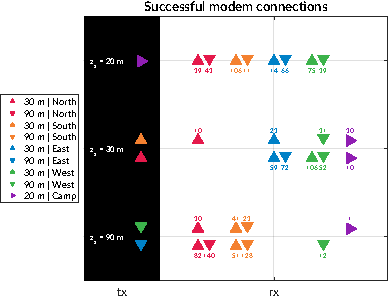
\includegraphics[width=.51\textwidth]{figs/Fig3a.pdf} \hfill
  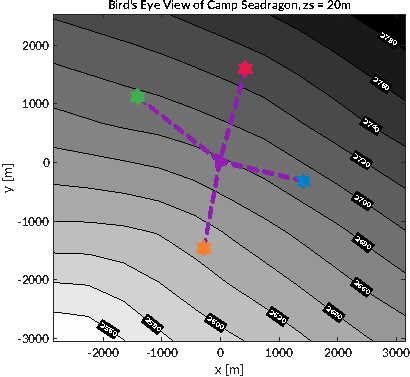
\includegraphics[width=.48\textwidth]{figs/Fig3b.pdf} \\
  \vspace{1em}
  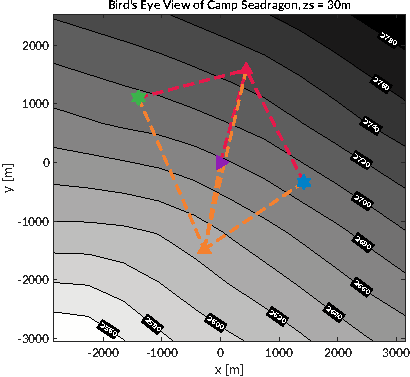
\includegraphics[width=.48\textwidth]{figs/Fig3c.pdf} \hfill
  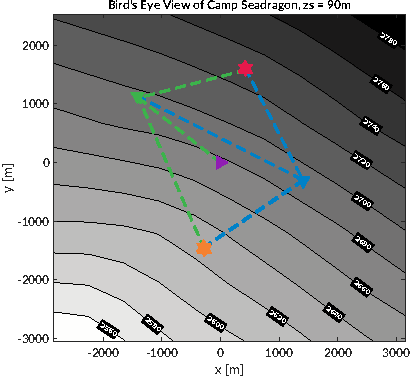
\includegraphics[width=.48\textwidth]{figs/Fig3d.pdf} \\
  \caption{An overview of the modem experiment by source and receiver depth and position. Subfigure (a) shows a chart of the successful events between source and receiver depth. The black column on the left, $tx$, shows the source depth, $z_s$. The column on the right, $rx$, shows the receivers with the amount of good contacts. The orientation of the triangles\textemdash sideways, upwards, and downwards\textemdash corresponds to depths of 20, 30, and 90 m. Subfigures (b-d) correspond to transmitter depths of 20, 30, and 90 m, respectively. Camp Seadragon, demarcated by the purple triangle, is situated just north of the continental shelf.}
  \label{fig:overview}
  \end{figure}

\clearpage

\subsubsection{Virtual layer}
The virtual layer describes the BELLHOP simulations for each communication event in the physical layer.
The SSP used for the raytracing is driven by a handful of weights applied to a basis function representation
of the SSP variability to reconstitute a number of realistic candidate SSPs \citep{leblanc_underwater_1980,lin_merging_2010}.
The SSP is the only human configurable input to the group velocity prediction.

During ICEX20, the SSP was toggled between the historical``baseline'' and a ``weighted'' estimate based on a local CTD cast, i.e. an optimal set of weights chosen by a human decision maker via an interactive Tactical Decision Aid framework \citep{bhatt_embedded_2021}.
For the post-processing analysis, we add the SSP from HYCOM for comparison, to mirror the information available on a submarine\textemdash modeled data, historical data, and \textit{in situ} data (personal conversation with LT B. Howard and LT CDR D. Goodwin). 
This order corresponds to increasing ducted conditions of the Beaufort Lens.

Fig. \ref{fig:raytrace-zs30} shows eigenrays in a range independent coordinate system for all three sound speed environments, for a source depth of 30 m.
It is important to note that BELLHOP produces an abundance of eigenrays; the ones displayed here are chosen by travel time proximity to the recorded data.
With this filter, the chosen eigenrays show a greater amount of surface interactions as the SSP duct conditions increase.

\begin{figure}[h!]
  \centering
  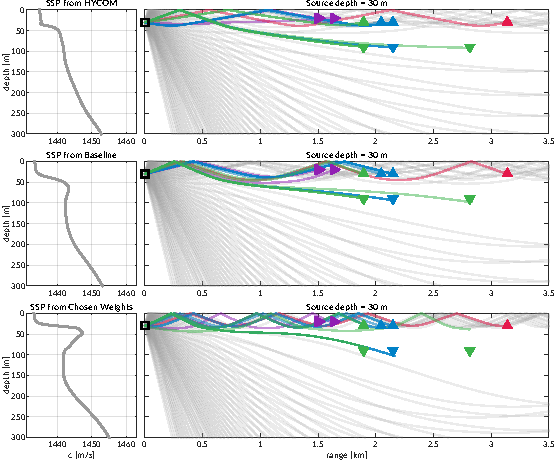
\includegraphics[width=\reprintcolumnwidth]{figs/Fig4.pdf}
  \caption{Eigenrays for beacon to beacon events for each sound speed with a nominal source depth of 30 m. The beacons are highlighted in color/marker coding in Fig. \ref{fig:overview}. The eigenrays are curated from BELLHOP by travel time proximity and are traced in the representative receiver colors over a total ray fan in gray.}
  \label{fig:raytrace-zs30}
  \end{figure}

\FloatBarrier
\subsection{Group velocity prediction methods}

The variation of horizontal group velocity from any source-receiver pair is the fundamental challenge to implement GPS-like navigation in an LBL navigation paradigm, especially in an acoustically complex propagation environment.
The use of the acoustic modem network for tracking relies on the accurate estimates of travel times between the submerged platform and range modems, supported by clock synchronization and a pre-determined scheduling of acoustic events.
For the Beaufort Lens in particular, the strong multipath effects make it virtually impossible to deterministically predict the modem triggering time.

\subsubsection{Minimal bounce criteria (MBC)}
Instead, for each individual node $i$, an embedded stochastic tracking framework is used to provide a running estimate of the horizontal group velocity $u_{i,j}$ for the conversion from travel time to range from modem $j$, with the ultimate goal of matching the naive group velocity, i.e. the GPS-recorded distance between two nodes divided by the modem-recorded one way travel time between them. 

In the ICEX20 configuration, the acoustic tracking is running on the topside computer, which controls the integrated communication and navigation range.
Here we assume that the group velocities $u_{i,j}$ are smoothly varying over the course of a vehicle mission, i.e., with respect to range, mission time, and the frequency of updates relative to vehicle motion. 
The group velocity is continuously tracked using predictions from the \textit{Virtual Ocean} infrastructure.

When the topside tracking framework receives a modem message, with a time delay, $\Delta t$, from one of the range modems, it will request a new estimate of the group velocity and its associated uncertainty.
The group velocity estimate is found using the vehicle's reported depth and the extrapolated navigation solution for range, $\hat{r}$, as inputs for the ray tracing program. The latter returns an impulse response estimate in the form of ray travel times $dt_{j}$ and amplitudes $a_{j}$ for that range and depth.

The initial call to BELLHOP is over a sparse local grid, from which the plane wave approximation is used to bring the ray to the range and depth posited by the onboard tracking solution.
For each grid point, BELLHOP will produce a number of arrivals resulting from multiple propagation paths for any source-receiver pair.
Using only the $N_0$ rays with neither surface nor bottom bounces, it will then estimate the current group velocity $u$ from a power weighted average of the ray travel times,
\begin{equation}
u = \frac{\hat{r} \sum_{n=1}^{N_{0}} a_{n}^{2}}{\sum_{n=1}^{N_{0}} dt_{n}a_{n}^{2}} ~, 
\end{equation}
and the associated weighted standard deviation,
\begin{equation}
\sigma_{u} \simeq \sqrt{\frac {\sum_{n=1}^{N_{0}} (dt_{n}-\hat{r}/u)^{2}a_{n}^{2}}{ \sum_{n=1}^{N_{0}} a_{n}^{2}} } \frac{u^{2}}{\hat{r}}
\end{equation}
If no direct paths exist, i.e. $N_{0}=0$, then the group velocity is computed using the same algorithm for the ray arrivals with one bounce, and so on.

Finally, the pseudorange is calculated simply as
\begin{equation}
r_{i,j} = u_{i,j} \Delta t_{i,j} 
\end{equation}

This stochastic method for group velocity calculation can run in real-time, appearing to be orders of magnitude faster than general post-processing methods which seek to determine the specific ray itself that best matches a prominent indicator from the arrival structure.
The method assumes direct path arrival, where multipath over the shallow receiver depth is trivial for the group velocity calculation; thus we call it the minimal bounce criteria (MBC).
The BELLHOP simulation that runs this calculation uses 3600 rays with launch angle fan of -60 to 60 degrees.
However, this high density of launch angles creates a greedy estimator of direct path eigenrays, and this simulation pipeline almost always guarantees a direct path found.
The MBC improves upon a deterministic estimate in that it considers the simplest ray path, travel time, and amplitude to predict a realistic group velocity.

\subsubsection{Nearest Bounce Criteria}

As shown in the eigenray traces of Fig. \ref{fig:raytrace-zs30}, an acoustic arrival does not always take the direct path from source to the receiver, and the path it takes is extremely dependent on the sound speed profile.
The suggested algorithm, the nearest bounce criteria (NBC), is a slight modification from the minimal bounce criteria, and includes multipath as a new dimension of information with negligible additional computation.
This metric was evaluated in post-processing.

Given a running estimate for the horizontal group velocity $u_{i,j}$ between nodes $i$ and $j$, the navigation system has an extrapolated value for range, $\hat{r}$, in the virtual layer, and a recorded travel time, $\Delta t_{i,j}$, in the physical layer.
Instead of using only the $N_0$ rays with neither surface nor bottom bounces to estimate group velocity and subsequently moving to incremental number of bounces only when no valid direct path solutions exist, we solve for the power weighted average of the ray travel time for the $N_k$ rays with $k$ bounces,
\begin{equation}
t_k = \frac{\sum_{n=1}^{N_{k}} dt_{n}a_{n}^{2}}{\sum_{n=1}^{N_{k}} a_{n}^{2}} ~, 
\end{equation}
find the nearest matching power weighted average to recorded travel time,
\begin{equation}
t_{i,j,k} = \min_{k=0,1,2,...} \left| t_k - \Delta t_{i,j} \right|
\end{equation}
predict a group velocity,
\begin{equation}
u_{i,j} = \dfrac{\hat{r}}{t_{i,j,k}}
\end{equation}
and estimate the range as was done previously.
\begin{equation}
r_{i,j} = u_{i,j}\Delta t_{i,j}
\end{equation}

This method selects a different group velocity based on the multipath arrival structure, as the detected arrival is not always the first arrival or the direct path and could even be masked by noise or blocked temporarily \citep{deffenbaugh_acoustic_1996}.
We manually cap the number of bounces to 4 because of the smaller operational scale and the attenuation accrued with many surface interactions.
Bottom bounces are not encoded separately because of ray's tendency to refract upward, not due to information limitations. 
In addition, for a more consistent comparison, the local sparse grid is standardized as 11$\times$11 points over 10 m in range and 20 m in depth, which is similar to those from the vehicle logs.
The extra size in depth addresses the computational limitations of how time-bounded eigenrays seem to stack vertically in the water column, as shown in Fig \ref{fig:rays3env-zs30}.

% =========================================================================== %
% =========================================================================== %

\FloatBarrier
\section{\label{sec:realtime} Real-time pseudorange results}

The modem experiment generated 811 beacon to beacon communication events with their own real-time MBC group velocity predictions.
As expected, the algorithm is generally overestimating range as it resolves a direct path that does not represent the actual arrival.
This section examines the absolute range error between the pseudorange and the GPS derived range with the caveat that the data collected is fairly unbalanced across source depths and sound speed conditions.

\begin{table}[h!]
\renewcommand{\arraystretch}{1.3}
\centering
\begin{tabular}{r|c|c|c|c|c}
SSP & Count & ~Mean [m] & ~Median [m] & ~STD [m] & ~Max [m] \\ \hline
Baseline & 243 & 11.38 & 11.96 & 4.23 & 23.95 \\ 
Chosen weights & 568 & 11.36 & 11.40 & 8.12 & 26.0 \\
\toprule
\end{tabular}
\caption[Range estimation error for \textit{in situ} events]{The range estimation error for \textit{in situ} events. The error here is presented as the absolute, not directional, error. Almost all directional errors, however, are positive.}
\label{tab:rangeErrorInSitu}
\end{table}

Table \ref{tab:rangeErrorInSitu} breaks down the number of events, mean, median, standard deviation, and maximum absolute range error for the \textit{in situ} calculations.
The mean and median for both sound speeds are similar on the order of centimeters; the chosen weights show a maximum 2 meters greater than that of baseline, but it is from a communication event that has no comparison in the baseline data set.
Analysis shows that where there is overlap in range between sound speed conditions used for the real-time MBC, the range error difference is no more than a few meters.
This is likely driven by the prominence of the duct.

The overarching statistical results show that both sound speed environments, given the smaller operational scales and shallow depths, are accurate enough to approximate the group velocity structure given the local grid.
Indeed, the error statistics indicated here are similar to those reported for the ICNN \citep{randeni_high-resolution_2021} and accurate enough to have facilitated a successful vehicle recovery.

\FloatBarrier
\section{\label{sec:postprocess} Post-processing pseudorange results}

There are 1242 total beacon to beacon events in the modem experiment that would have been accepted by the ICNN for real-time ranging and navigation had the ranging behavior been running for all modems in the network, and not only for tracking the vehicle.
A post-processing analysis that replicated the real-time pipeline was run to overcome the unequal distribution of communication events with respect to depth, range, and sound speed status.

It is important to note that the value for the extrapolated range, $\hat{r}$, is only tracked when the modem runs the vehicle behavior; thus we replace $\hat{r}$ with the GPS-tracked range for all modem events.
Because $\hat{r}$ converges to the correct solution, a comparison of $\hat{r}$ with the GPS-tracked range shows a normal, zero-centered distribution within the bounds of GPS drift.
The present analysis therefore seeds realistic but ``omniscient'' knowledge of the extrapolated range and leverages the post-processing pipeline to more thoroughly evaluate the acoustic range estimate for all modem events, with three relevant sound speed sources, and both group velocity criterion.
Accordingly, the results in this section evaluate the utility of the algorithms and sound speed sources, divorced from their role in the ICNN while maintaining real-time relevance.

\FloatBarrier
\subsection{Group velocity predictions}

The minimal and nearest bounce algorithms are applied, both without the plane wave extensions, with the three sound speed inputs shown in Fig.~\ref{fig:raytrace-zs30}.
The resulting predicted group velocities for a source depth of 30 m are shown in Fig~\ref{fig:gvel30}.
The takeaways from this source depth are representative of those from 20 and 90 m as well (see Supplementary Fig.~\ref{fig:gvelMore}).

\begin{figure}[h!]
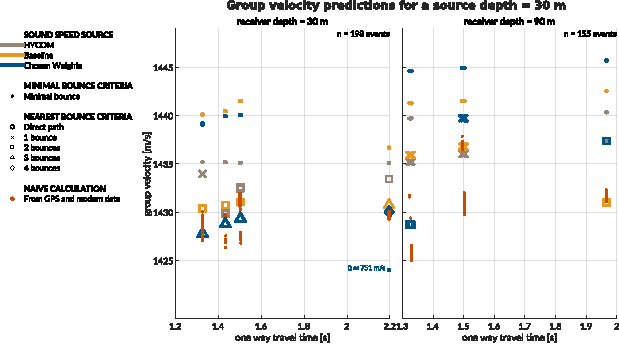
\includegraphics[width=\columnwidth]{figs/Fig5.pdf}
\caption{A comparison of group velocity predictions for all beacon to beacon events in post-processing with a source depth of 30 m, with group velocity on the y-axis and recorded travel time on the x-axis. The left panel is for a receiver depth of 30 m; the right panel for 90 m. The sound speed source is indicated by color. The minimal and nearest bounce criterion are distinguished by different marker shapes, compared to the separately colored red dots showing the naive, data-driven group velocity calculation.}
\label{fig:gvel30}
\end{figure}

Because direct path dominates the predictions from the MBC, group velocity estimates are greater than those from NBC.
The one instance this is not true is important to mention\textemdash for a travel time of 2.2 s, where the minimal multipath is dominated by a single bottom bounce (the red line to the furthest transmission in Fig. \ref{fig:raytrace-zs30}, more detail in Section \ref{subsec:anomalousBeacon}).
The nearest bounce method never classifies anything as direct path for the 30 m source, though BELLHOP is quite adept at finding those rays. 

The goal of the group velocity estimation is to converge towards the naive group velocity estimation, i.e. the GPS-derived range divided by the recorded travel time.
For a 30 m receiver depth, the NBC shows more overlap with data-derived values as it classifies multipath more correctly.
For a 90 m receiver depth, the overlap is less accurate due to computational constraints of a limited fan of rays entering the shadow zone rendering a less reliable simulated times of arrival packet.

Overall, analysis shows that the higher multipath classification produces more accurate range estimates, likely driven by a tighter bundle of rays.
However, that data is too small to draw significant conclusions.
Discontinuities in multipath classification verify our hypothesis for its importance to a smoothly varying group velocity, as shown in the cluster for a receiver depth of 30 m, where HYCOM jumps from one to two bounces amidst the baseline SSP and weighted SSP smoothly increasing while consistently seeing two and three bounces, respectively.

\FloatBarrier
\subsection{Pseudorange error versus one way travel time}

Fig. \ref{fig:rangeError} shows the directional range error footprints for all three sound speed inputs with respect to OWTT, separated by source and receiver depth configurations.
The weighted SSP range error generally has the smallest and most zero-centered footprint.
The one case it does not is for the source-receiver pairings between 30 and 90 m in depth.
The increased error for these reciprocal transmission paths is most likely driven by the computational artifacts encountered when propagating through the steep sound speed gradients of the lens and through the shadow zone.
All other source depth pairings are significantly improved using the chosen weights compared to HYCOM or the baseline.

When using a linear scaling to convert travel time into range, any offset between the assumed sound speed and the horizontal group velocity produces unconstrained error with increasing receiver distance.
Most importantly, we see the consequences of the adaptive group velocity in that range error does not strictly increase with OWTT.

\begin{figure}[!ht]
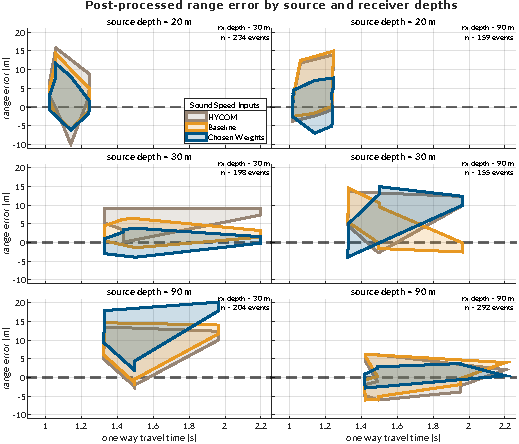
\includegraphics[width=\textwidth]{figs/Fig6.pdf}
\caption{The post-processed range error for source depths of 20, 30, and 90 m, and receiver depths of 30 and 90 m. The dashed gray line shows no error. The shaded region connects the range performance across all events.}
\label{fig:rangeError}
\end{figure}

\FloatBarrier
\subsection{Pseudorange estimations from the nearest and minimal bounce criteria}

The previous section displayed the pseudorange performance using the NBC.
Here, we explicitly compare the ranging accuracy between the nearest and minimal bounce criteria for all events in the post-processing pipeline.
It is important to note that because the post-processing pipeline is the same for both methods, that the efficacy of the NBC compared to the MBC is 100\%, as the former simplifies to the latter for direct path classifications.

\begin{figure}[h!]
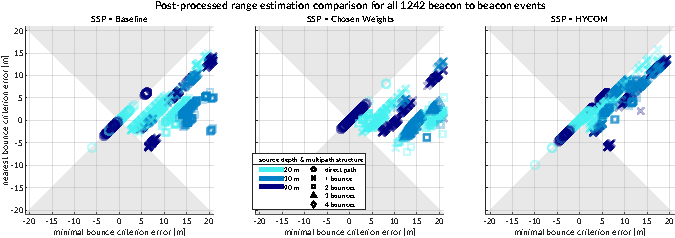
\includegraphics[width=\textwidth]{figs/Fig7.pdf}
\caption{\label{fig:compareV1V2}{A comparison of range estimation error for all beacon to beacon events in post-processing. From left to right, the SSPs are the baseline, the chosen weights, and HYCOM. The colors indicate the source depth, darkening with depth, and the shapes indicate the multipath structure. Because this plot is square, the shaded region shows where the updated algorithm is less accurate than the \textit{in situ} algorithm.}}
\end{figure}

Figure \ref{fig:compareV1V2} is a crossmap for all three SSPs for both group velocity predictors, with the minimal bounce on the x-axis and the nearest bounce on the y-axis; the important range estimation metrics are summarized in table \ref{tab:rangeErrorV1V2}.

All the events are on the unshaded region of the plots\textemdash the MBC has a systemic overestimation, which is reduced via NBC as events straddle the x-axis.
The improvement from MBC to NBC is most evident for the realistic sound speed; while the HYCOM SSP improves from a median absolute range error of 6.41 to 4.61 m, the baseline SSP improves from 10.30 to 2.27 m, and the weighted SSP improves from 13.28 to 2.12 m.
Table \ref{tab:rangeErrorPost} shows further statistics on the absolute range error by SSP and group velocity algorithm.
The order of magnitude improvement in the ducted SSPs demonstrate the effectiveness of the algorithm exploiting the multipath conditions.

Given the computational constraints of real-time modeling, the gridded approach facilitates enough multipath classification to build in a ``ray ensemble'' of characteristic group velocities.
This result is not always possible when aiming to find eigenrays to just an individual point, even with a higher density of launch angles.
An important takeaway for those interested in ray-based localization is leveraging a local grid to give BELLHOP tolerance for finding solutions that otherwise may not be found in a center or single point solution.
The limitations of numerical computation, particularly for a complex environment, are more adeptly addressed by accepting some uncertainty in position than by prescribing an exact solution.
Even though BELLHOP is a greedy estimator for eigenrays, the additional data created is a negligible burden. 

\begin{table}[h!]
\renewcommand{\arraystretch}{1.5}
\centering
\begin{tabular}{r|cc|cc|cc}\toprule
 & \multicolumn{2}{c|}{\textbf{Baseline} } & \multicolumn{2}{c|}{\textbf{Chosen Weights} } & \multicolumn{2}{c}{\textbf{HYCOM}} \\
 algorithm & \cellcolor[HTML]{EFEFEF}minimal & nearest & \cellcolor[HTML]{EFEFEF} minimal& nearest & \cellcolor[HTML]{EFEFEF}minimal & nearest \\ \hline
 minimum [m] 	& \cellcolor[HTML]{EFEFEF}0.01 & 0.00	& \cellcolor[HTML]{EFEFEF}0.00 	& 0.00 	& \cellcolor[HTML]{EFEFEF}0.11 & 0.01 \\
 25th \% [m]   & \cellcolor[HTML]{EFEFEF}4.96 & 0.99	& \cellcolor[HTML]{EFEFEF}6.26 	& 0.95 	& \cellcolor[HTML]{EFEFEF}3.30 & 2.25 \\   
 median [m]		& \cellcolor[HTML]{EFEFEF}10.30 & 2.27 	& \cellcolor[HTML]{EFEFEF}13.28 & 2.12 	& \cellcolor[HTML]{EFEFEF}6.41 & 4.61 \\
 75th \% [m]   & \cellcolor[HTML]{EFEFEF}15.81 & 5.51 	& \cellcolor[HTML]{EFEFEF}19.75 & 4.11 	& \cellcolor[HTML]{EFEFEF}10.92 & 7.46 \\
 maximum [m]    & \cellcolor[HTML]{EFEFEF}22.52 & 14.96 & \cellcolor[HTML]{EFEFEF}1491  & 20.21 & \cellcolor[HTML]{EFEFEF}19.55 & 15.81 \\
 \toprule
\end{tabular}
\caption[Comparison of post-processing range estimation algorithms across all events]{A comparison of range estimation metrics for each sound speed source and group velocity estimation algorithm for all 1283 beacon to beacon events via post-processing. The 0th (minimum), 25th, 50th (median), 75th, and 100th (maximum) percentiles are shown to the range resolution afforded by the WHOI Micro-Modem. There are a few outliers that drive the mean to be higher than the median.}
\label{tab:rangeErrorV1V2}
\end{table}

All plots in Fig. \ref{fig:compareV1V2} show the same 45 degree banding of source depth and multipath structure, indicating systemic GPS noise.
The width of those bands indicates the high precision of the acoustic methods relative to lower precision from GPS.
Some bands are adjacent to others of the same styling, likely due to ice drift and/or various GPS satellite constellations.

\FloatBarrier
\subsection{Further analysis of the anomalous beacon to beacon connection}
\label{subsec:anomalousBeacon}

As shown in table \ref{tab:rangeErrorPost}, there is a striking maximum range error of 1491 m for the weighted SSP in the minimal bounce criteria.
This section isolates the events that encompass that outlier for further examination, summarized in table \ref{tab:rangeErrorPostExplanation}.
There are 10 events from South transmitting at 30 m depth to North receiving at 30 m depth.
The OWTT spread is from 2.1958 to 2.1963 s; the naive group velocity is 1429.3 to 1430.1 m/s; and the GPS-tracked range is from 3138.54 m to 3140.87 m.
This example ends up being an excellent case study for how sound speed and multipath fidelity work in concert to minimize range error.

\begin{table}[h!]
\renewcommand{\arraystretch}{1.5}
\centering
\begin{tabular}{r|cc|cc|cc}\toprule
 & \multicolumn{2}{c|}{\textbf{Baseline} } & \multicolumn{2}{c|}{\textbf{Chosen Weights} } & \multicolumn{2}{c}{\textbf{HYCOM}} \\
 algorithm & \cellcolor[HTML]{EFEFEF}minimal & nearest & \cellcolor[HTML]{EFEFEF} minimal& nearest & \cellcolor[HTML]{EFEFEF}minimal & nearest \\ \hline
 \# bounces 				& \cellcolor[HTML]{EFEFEF}1 		& 3 		& \cellcolor[HTML]{EFEFEF}1 		& 4 		& \cellcolor[HTML]{EFEFEF}0 	 & 2 \\
 mean OWTT [s] 				& \cellcolor[HTML]{EFEFEF}2.1853 	& 2.1943 	& \cellcolor[HTML]{EFEFEF}4.1812 	& 2.1955 	& \cellcolor[HTML]{EFEFEF}2.1877 & 2.1902 \\
 mean group velocity [m/s] 	& \cellcolor[HTML]{EFEFEF}1436.7 	& 1430.8 	& \cellcolor[HTML]{EFEFEF}750.88 	& 1430.0 	& \cellcolor[HTML]{EFEFEF}1435.1 & 1433.4 \\
 range error [m] 			& \cellcolor[HTML]{EFEFEF}15.4 		& 2.39 	 	& \cellcolor[HTML]{EFEFEF}-1491 	& 0.77 		& \cellcolor[HTML]{EFEFEF}11.9 & 8.30 \\
 \toprule
\end{tabular}
\caption[Further look at algorithm differences for one beacon to beacon pairing]{A comparison of range estimation metrics for each sound speed source and group velocity estimation algorithm on all 10 communication events between North at 30 m \& South at 30 m.}
\label{tab:rangeErrorPostExplanation}
\end{table}

The large error in this instance is driven by the MBC unexpectedly defaulting to a bottom bounce with a much greater OWTT.
The NBC classifies the multipath as 4 bounces, reducing the range error from greater than a kilometer to less than a meter.
While there is no actual way of knowing if this is the correct multipath structure, the range error is remarkably small, at 0.025\%. 
This pattern of not choosing the minimal observed bounce structure is consistent across all SSPs; the baseline goes from 1 to 3 bounces and HYCOM goes from 0 to 2 bounces.
Notably, the baseline and HYCOM range errors are never egregiously large, but are nonetheless improved with the NBC algorithm.
Thus, for acoustically complex environments, the NBC has a disproportionately positive impact as the estimated SSP approaches the desired SSP.

\FloatBarrier
\subsection{GPS sensor drift at polar latitudes}

Systemic GPS drift drives the severe banding found in comparisons of range estimations via both group velocity algorithms, as shown in Fig. \ref{fig:compareV1V2}, with those bands showing 100\% positive correlation between methods and being a similar size in meters.
Thus, while this work is primarily motivated by achieving similar accuracy and precision of GPS, the impressive results from acoustic ranging necessitate a discussion about the limitations of GPS, particularly at polar latitudes.

The ``Global Positioning System Standard Positioning Service Performance Standard'', published by the Department of Defense in Apr 2020 claims that well-designed GPS receivers have been achieving a horizontal accuracy of 3 meters and a vertical accuracy of 5 meters, 95\% of the time.
But ``well-designed'' is an ambiguous enough term that obfuscates two confounding factors for high latitude GPS drift\textemdash operational limitations and ionospheric scattering.

% operational
There are two metrics that demonstrate the operational limitations of GPS tracking technologies\textemdash fix rate and positional dilution of precision (PDOP) \citep{swanlund_gps_2016}.
Fix rate looks at the ratio of successful fixes to overall attempts in acquiring a location.
In animal tracking studies in polar latitudes, fix rates have significantly improved in the last twenty years, from as low as 26\% in 1996 \citep{moen_effects_1996} to 87.2\% in 2018 \citep{jung_accuracy_2018}.
The latter study showed a precision of 4.3 $\pm$ 4.0 m and an accuracy of 6.0 $\pm$ 4.7 m.
While fix rate is a significant metric to evaluate GPS robustness, it is accuracy and precision, and not the fix rate, that explain the severe banding observed; fix rate bias, where various aspects of a landscape can induce bias by impeding the GPS receiver from acquiring its location, is not relevant given the static nature and small time window of ICEX20.

PDOP looks at the effect of satellite geometry on location precision, as satellite orbits are designed to optimize performance for human population density.
A high PDOP value indicates a poor geometric configuration, such as satellites being tightly clustered above a GPS receiver, that limits the reliability of trilateration.
The literature shows correlation between PDOP values and location error \citep{swanlund_gps_2016}.
PDOP is generally thought of as three-dimensional positioning and can be broken down into the horizontal and vertical components, HDOP and VDOP, respectively.
The low elevation angles in polar areas are good for horizontal positioning but are susceptible to poorer vertical positioning.
Overall this contributes to higher noise level in observations than usually seen in most global applications.
The sparse and limited infrastructure in the Arctic make it ideal for satellite-based navigation, with some research proposing new satellite systems to accommodate increased interest in the region \citep{reid_gnss_2016}.

However, both of these metrics are functions of the satellite constellation available to any given GPS receiver.
The Arctic is beyond the reach of many geostationary satellites, where they are low on the horizon and only visible for brief periods.
Given that their positions are tracked by stations on Earth, and their timing is updated twice a day via atomic clock, a reasonable hypothesis for bands of GPS error are different and/or updated satellite connections.

% ionospheric
The second confounding factor is the ionosphere, the layer of the Earth's atmosphere roughly 80 to 1000 km above the surface that contains a high concentration of ions and free elections. 
In the ionosphere, electromagnetic signals are affected by the total amount of electrons encountered by the signal; the size of the signal delay is dependent on the carrier frequencies.
The literature even references the total amount of electrons encountered by the ``GPS raypath'' as a means of explaining signal fluctuations \citep{themens_nature_2015}.
This variability is observed by seasonal and solar cycle variabilities \citep{themens_nature_2015}, severe ionospheric storms \citep{mitchell_gps_2005}, and auroral activity (increased electron precipitation) \citep{jin_gps_2014,gwal_gps_2011}.
In fact, the \textit{aurora borealis} was observed on multiple nights during ICEX20.

In a humbling twist, at polar latitudes, GNSS systems experience similar operational, technical, and environmental challenges that we observe in underwater acoustic communications.
Figure \ref{fig:gps-drift-example} highlights the GPS and observed OWTT drift relative to the ice movement for two pairs of modem buoy connections.
The two panels indicate the GPS drift as $\delta R = \sqrt{\delta x^2 + \delta y^2}$ and temporal drift, $\delta t$, relative to the median OWTT recorded between the two modems.
The dashed line is scaled by a group velocity of 1440 m/s, such that if there were ideal sensor measurements with no drift, all events should exist on or near the line.

\begin{figure}[h!]
	\centering
	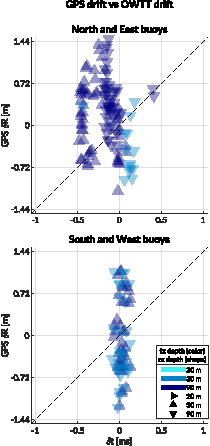
\includegraphics[width=\reprintcolumnwidth]{figs/Fig8.pdf} 
	\caption{A comparison of GPS drift (y-axis) versus OWTT drift (x-axis), colored by source and receiver depth. The physical link between North and East are shown on the top; South and West is on the bottom.}
	\label{fig:gps-drift-example}
\end{figure}

The top panel shows the connections between the North and East buoys.
There is relative, i.e. non-rigid, ice movement between the North and East buoys, evidenced by events spanning the dashed line.
But the height of the scatter plot is indicative of the precision of the GPS signal, as it remains consistent across many arrival time bands.
Naturally, some minor offsets between these vertical bands relate to different operational configurations of source and receiver depth.
However, the large majority of events show vertical banding for the same nominal $\delta t$, indicating the amount of GPS drift.

This idea of GPS drift relative to the same OWTT measurements is further indicated by events between the other two buoys, South and West, in the bottom panel.
These buoys are moving in a more rigid ice floe and there is minimal impact by source and receiver depth on the spread of OWTT.
The GPS drift is much larger relative to the OWTT drift, which is sensitive to acoustic scattering, multipath, and/or environmental microstructure.

These are just two subsets of the physical links that cover all four GPS modem buoys.
The GPS at camp is the least accurate due to the human activity and infrastructure occluding the physical puck.

% =========================================================================== %
% =========================================================================== %
\section{\label{sec:discussion} Discussion}

Range estimation is an essential step of acoustic localization and navigation.
Current approaches in real-time underwater acoustic navigation simplify the non-linear relationship between a sound speed profile and acoustic propagation with a deterministic sound speed.
Some post-processing approaches attempt to leverage the acoustic arrival structure via various ray methods, but often use a singular SSP for simplicity, even over long term missions or dynamic conditions.
Thus, the conversion from travel time to range, particularly for real-time vehicle deployments, can be pre-conditioned for error growth as the OWTT/range increases.

For GPS-denied navigation, especially in hostile environments like the Arctic, tolerance for error is close to none.
This work addresses a critical need in acoustic navigation by retooling acoustic arrival methods generally deemed too complex or labor intensive for real-time, ray-based range estimation to achieve GPS-like positioning.

We hypothesize and validate that the embedded stochastic prediction of a single group velocity is a smoothly varying function of range, source and receiver depth pairings, as well as multipath structure.
We employ a GPS-tracked experiment to have a ground truth comparison for real-time localization algorithms.
The real-time system achieves GPS-like navigation for an AUV without taking into account multipath structure; the ranging error improves by an order of magnitude with the suggested multipath adaptability, minimizing range error to single meters.
Post-processing analysis shows that this method of ranging is sensitive to GPS drift itself; thus embedding a stochastic prediction of the horizontal group velocity has an outsized benefit to minimizing trilateration error.

There are many avenues through which this approach can be further refined and tested for field operations.
Amongst them is defining the uncertainty grid for BELLHOP via stochastic or data-driven measures such as the distance traveled by the AUV between ICNN updates or the magnitude of the position corrections by the ICNN.
Another is to entirely remove the seeded range and instead rely on the submerged asset's depth and recorded OWTT to find high probability fields in range.

The literature in underwater acoustic navigation and positioning is either real-time or physics-based.
In this paper we demonstrate a field-tested approach that is both real-time and physics-based; this is achieved by coupling data streams with fast acoustic modeling.
The methods exploit the upward refracting nature and the total ice cover of the Arctic environment to achieve remarkable ranging accuracy and precision.
It transforms multipath, widely considered as an obstacle for acoustic ranging, into a new information content to refine ranging accuracy.
We believe that this work enables more accurate range estimation, localization, and/or navigation for any field experiment given known source and receiver depths.

\subsection{Broader relevance \& future work}

Performance in other acoustic environments may require introducing a different thresholded metric to sort time of arrivals.
Given the NBC algorithm's improvement with increased multipath, its effectiveness is likely only challenged by the valid operational scales of a range independent propagation environment.
For mesoscale operations, like that of many gliders, the group velocity criteria may need to be modified to better account for variability driven by range dependent propagation through internal waves, eddies, or even bathymetric changes like underwater volcanoes.
BELLHOP simulations provide other relevant eigenray information, like time and angle of arrival, that is ripe for statistical and machine learning methods to classify a representative group velocity.
A bespoke and fast ray tracing method, which was used during ICEX20 to evaluate the acoustic fit of sound speed profile parameterization \citep{bhatt_embedded_2021}, can easily report back the number of turning points instead of the number of bounces for multipath classification.

This approach will start to break down in extremely dynamic environments.
Fast moving fronts, as seen in estuaries like the Connecticut River into the Long Island Sound, present an entirely new set of challenges not seen by internal waves or eddies.
Buoyancy fluctuations in these regions threaten even simple AUV tasks like following a trackline.
Acoustic communications are further complicated given a shallow environment with significant scattering \citep{lavery_measurements_2010,ross_acoustic_2012,lavery_broadband_2013}, where fast acoustic modeling may only be coherent for trivial probabilities of the ocean state.
Realistic \textit{in situ} considerations of the acoustic environment may not be possible in such environments without complete through-the-sensor integration of echosounder data and/or a hyper-realistic onboard ocean model.

Many approaches to underwater navigation combine it with acoustic tomography, i.e., a joint estimation of both source and receiver locations and the ocean volume between them.
There has been considerable success at this effort in post-processing methods, which utilize intensive\textemdash and due to the non-linearity of sound propagation, often brute force\textemdash computational methods. 
For vehicle operations, fast tomography is the ideal implementation, in that one can fully consider how sound speed structure, horizontally and vertically, influences sound propagation.
AUVs can serve as moving sources to better image the ocean volume \citep{deffenbaugh_optimal_1997,elisseeff_ocean_2002}, where mobile tomography and navigation converge on the same set of component technologies: position estimation, sound speed parameterization estimation, ray path identification, and vehicle path optimization.

But there are overwhelming challenges, operationally and computationally, for fast, mobile tomography to become a realistic endeavor.
Addressing the spatial and temporal scales of what can be solved deterministically and what must be solved stochastically imposes a resolution constraint on the utility of gridded models\textemdash resolving fine features inaccurately (or with a false sense of confidence) could be more harmful than assuming range independence.
Given that AUV operations are often on small spatial and temporal scales, the added benefit of a gridded model is quite small, and in cases like the Arctic, may actually mischaracterize the ocean volume. 
For gliders, with longer and larger operational scales, an ocean model may provide more useful information.
Currently gliders are low power and do not have the storage or computational power to run a full-scale, realistic ocean model.
A lightweight representation of the key environmental and acoustic features, passed through the same manner of acoustic message from the modem experiment, may drastically improve glider navigation.

The Arctic, a generally inaccessible, dangerous, and expensive region for crewed monitoring via icebreakers,  is a prime location to invest in vehicle deployments and underwater observatories \citep{mikhalevsky_multipurpose_2015}.
As anthropogenic climate change renders the region more accessible, safe navigation infrastructure and practices will be increasingly vital for industry, tourism, commercial, and military operations.
We hope this work enables more frequent and confident monitoring for remote and/or dangerous regions of high climate security importance.

\clearpage
\section*{Supplementary Figures}

\subsection*{Ice movement during the modem experiment}
\begin{figure}[h!]
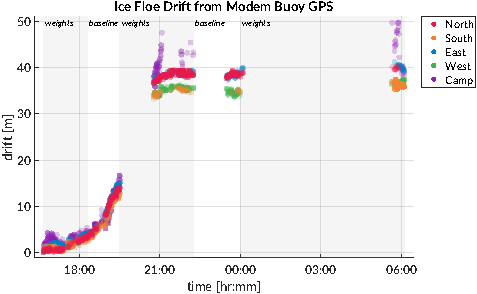
\includegraphics[width=\textwidth]{figs/Fig9.pdf}
\caption{\label{fig:iceFloeDrift}{The ICNN accounts for ice drift throughout the mission duration. This is the magnitude of the ice drift recorded, at each buoy, throughout the modem experiment. The shaded regions reference which sound speed estimate was used.}}
\end{figure}

\clearpage
\FloatBarrier
\subsection*{Group velocity prediction by source depth}
\begin{figure}[h!]
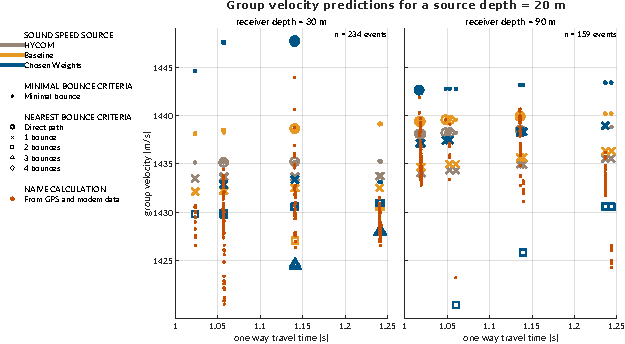
\includegraphics[width=0.8\textwidth]{figs/Fig10a.pdf} \\
\vspace{2em}
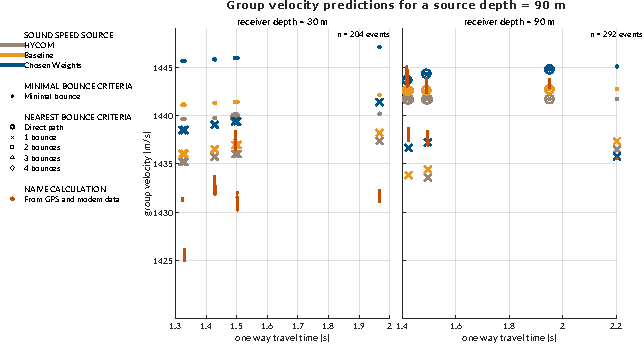
\includegraphics[width=0.8\textwidth]{figs/Fig10b.pdf}
\caption{A comparison of group velocity predictions for all beacon to beacon events in post-processing. The top panel shows a source depth of 20 m; the bottom panel shows a source depth of 90 m. The sound speed source is indicated by color. The minimal and nearest bounce criterion are distinguished by different marker shapes, compared to the separately colored orange dots showing the naive, data-driven group velocity calculation.}
\label{fig:gvelMore}
\end{figure}

% ================================================== %
% \begin{figure}[ht]
% \includegraphics[width=\reprintcolumnwidth]{figsamp.jpg}
% \caption{\label{fig:FIG1}{Caption here.}}

% \raggedright
% {\color{red}
% Note: The only figure formats allowed are the following:
% .pdf, .ps, .eps, or .jpg. Figure files must be named in this fashion:
% Figure\#.xxx, where ``\#'' is the figure number and ``xxx'' is the file format
% (Figure1.eps, Figure2.jpg, Figure3a.ps, Figure3b.ps, etc).
% }

% [For these sample pages we have used only figsamp.jpg for convenience]
% \end{figure}
% ================================================== %
\FloatBarrier
\clearpage
\begin{acknowledgments}
We acknowledge the significant operational effort spearheaded by the LAMSS ICEX20 team and all our collaborators.
Bhatt was funded by a National Defense, Science, and Engineering Graduate Fellowship.
This work was supported by the Office of Naval Research 322-OA under ICEX20 (N00014-17-1-2474) and Task Force Ocean (N00014-19-1-2716).

\end{acknowledgments}

\bibliography{sampbib}
